\subsection{MPP tracking solar charging controllers}
The aim of a SCC is to distribute a PV generator's electrical energy to supply one or more electrical consumers and to recharge an electrochemical energy storage device. The latter is required to supply electrical consumers during times without sunlight. SCCs that can track the MPP of a PV generator, thus providing the greatest electrical energy to the load and the electrochemical energy storage device (compare to figure \ref{fig:tikz/tikz_solar_energy_distribution}), determine the current $I_{\mathrm{MPP}}(\vartheta_{\mathrm{C}}, \Phi_{\mathrm{G}})$ and voltage $U_{\mathrm{MPP}}(\vartheta_{\mathrm{C}}, \Phi_{\mathrm{G}})$. This can be accomplished by analyzing the equation (\ref{eq:p_pv_i}) from which the derivative of $P_{\mathrm{PV}}(I_{\mathrm{PV}}, \vartheta_{\mathrm{C}}, \Phi_{\mathrm{G}})$, with respect to $I_{\mathrm{PV}}$, results in the equation (\ref{eq:dp_pv}).
	\begin{equation} \label{eq:dp_pv}
	\centering
		 \dfrac{\mathrm d P_{\mathrm{PV}}(I_{\mathrm{PV}}, \vartheta_{\mathrm{C}}, \Phi_{\mathrm{G}})}{\mathrm d I_{\mathrm{PV}}} = m \, N_{\mathrm{C}} \, U_{\mathrm{T}} \left( \ln \left( \frac{I_{\mathrm{Ph}} - I_{\mathrm{PV}} + I_{\mathrm{S}}}{I_{\mathrm{S}}} \right) - \frac{I_{\mathrm{PV}}}{I_{\mathrm{Ph}} - I_{\mathrm{PV}} + I_{\mathrm{S}}} \right)
	\end{equation}
Since the slope of the curve $P_{\mathrm{PV}}(I_{\mathrm{PV}}, \vartheta_{\mathrm{C}}, \Phi_{\mathrm{G}})$ becomes $0\mathrm{V}$ for its maxima, $I_{\mathrm{PV}} = I_{\mathrm{MPP}}$ applies as shown below:
	\begin{equation} \label{eq:dp_pv_zero}
	\centering
		 m \, N_{\mathrm{C}} \, U_{\mathrm{T}} \left( \ln \left( \frac{I_{\mathrm{Ph}} - I_{\mathrm{MPP}} + I_{\mathrm{S}}}{I_{\mathrm{S}}} \right) - \frac{I_{\mathrm{MPP}}}{I_{\mathrm{Ph}} - I_{\mathrm{PV}} + I_{\mathrm{S}}} \right) = 0\mathrm{V} \text{.}
	\end{equation}
If now the equation (\ref{eq:dp_pv_zero}) is subtracted from the equation (\ref{eq:u_of_i}) for the case $U_{\mathrm{PV}}(I_{\mathrm{MPP}}, \vartheta_{\mathrm{C}}, \Phi_{\mathrm{G}}) = U_{\mathrm{MPP}}(\vartheta_{\mathrm{C}}, \Phi_{\mathrm{G}})$, the voltage at MPP can be rewritten as follows \cite{Mertens:2015, Wagner:2018}:
	\begin{equation} \label{eq:u_mpp_i_mpp}
	\centering
		 U_{\mathrm{MPP}}(I_{\mathrm{MPP}}, \vartheta_{\mathrm{C}}, \Phi_{\mathrm{G}}) = \frac{m \, N_{\mathrm{C}} \, U_{\mathrm{T}} \, I_{\mathrm{MPP}}}{I_{\mathrm{Ph}} - I_{\mathrm{MPP}} + I_{\mathrm{S}}} \text{.}
	\end{equation}

In addition to the equation (\ref{eq:p_mpp}), $P_{\mathrm{MPP}}(\vartheta_{\mathrm{C}}, \Phi_{\mathrm{G}})$ can directly be obtained from $\Phi_{\mathrm G}$ as presented in the equation (\ref{eq:p_mpp_phi_temp}). For this, however, the PV generator's \emph{efficiency} $\eta_{\mathrm{PV}}$ in $\left(1\right)$ and its temperature coefficient $\mathrm{TC}(P_{\mathrm{MPP}})$ in $\left( \% ^\circ \mathrm{C}^{-1}\right)$ for the electrical power output at MPP must be known.\footnote{Typical $\mathrm{TC}(P_{\mathrm{MPP}})$ values for Si-PV cells are around $-0,4$ to $-0,5$ $\% ^\circ \mathrm{C}^{-1}$.} These quantities can be found in the data sheet of a PV generator. 
	\begin{equation} \label{eq:p_mpp_phi_temp}
	\centering
		 P_{\mathrm{MPP}}(\vartheta_{\mathrm{C}}, \Phi_{\mathrm{G}}) = \eta_{\mathrm{PV}} \, \Phi_{\mathrm G} \left[ 1 + \frac{\mathrm{TC}(P_{\mathrm{MPP}})}{100\%} \left(\vartheta_{\mathrm{C}} - \vartheta_{\mathrm{STC}} \right) \right]
	\end{equation}
Alternatively, $\eta_{\mathrm{PV}}$ can be calculated by using the equation (\ref{eq:p_mpp_phi_temp}) and the table \ref{tab:table_STC}, while regarding the expression $P_\mathrm{MPP,STC} = U_\mathrm{MPP,STC} \, I_\mathrm{MPP,STC}$. This is because $\eta_{\mathrm{PV}}$ depends exclusively on the material and the structure of a PV cell. Moreover, it is assumed that the PV cell is ideal and that every photon which hits the semiconductor and fulfills $W_{\mathrm{Ph}} > \Delta W_{\mathrm{gap}}$, is absorbed and leads to an electron which contributes to $I_\mathrm{Ph}$. In the mentioned inequality $W_{\mathrm{Ph}}$ is the \emph{energy of a photon} in $\left(\mathrm{eV}\right)$ and $\Delta W_{\mathrm{gap}}$ is the \emph{band gap} in $\left(\mathrm{eV}\right)$ of the semiconductor \cite{Mertens:2015, Wagner:2018}.

With the equations (\ref{eq:p_mpp}), (\ref{eq:u_mpp_i_mpp}) and (\ref{eq:p_mpp_phi_temp}), the PV generator's current at MPP can be converted into the following quadratic equation:
	\begin{equation} \label{eq:i_mpp_quadratic}
	\centering
		 I_{\mathrm{MPP}}^2 + c_{\mathrm{PV}} \, I_{\mathrm{MPP}} - c_{\mathrm{PV}} \left(I_{\mathrm{Ph}} + I_{\mathrm{S}}\right) = 0\mathrm{A}^2 \text{, }
	\end{equation}
with $c_{\mathrm{PV}}$ being:
	\begin{equation} \label{eq:c_pv}
	\centering
		 c_{\mathrm{PV}} = \dfrac{\eta_{\mathrm{PV}} \, \Phi_{\mathrm G} \left[ 1 + \dfrac{\mathrm{TC}(P_{\mathrm{MPP}})}{100\%} \left(\vartheta_{\mathrm{C}} - \vartheta_{\mathrm{STC}} \right) \right]}{m \, N_{\mathrm{C}} \, U_{\mathrm{T}}} \text{.}
	\end{equation}
Finally, $I_{\mathrm{MPP}}(\vartheta_{\mathrm{C}}, \Phi_{\mathrm{G}})$ can be solved to:
	\begin{equation} \label{eq:i_mpp_sqr_root}
	\centering
		 I_{\mathrm{MPP}}(\vartheta_{\mathrm{C}}, \Phi_{\mathrm{G}}) = \sqrt{\frac{c_{\mathrm{PV}}^2}{4} + c_{\mathrm{PV}} \left(I_{\mathrm{Ph}} + I_{\mathrm{S}}\right)} - \frac{c_{\mathrm{PV}}}{2} \text{.}
	\end{equation}
The PV generator's voltage at MPP can consequently be calculated using the equation (\ref{eq:i_of_u}) for the case $U_{\mathrm{PV}}(I_{\mathrm{MPP}}, \vartheta_{\mathrm{C}}, \Phi_{\mathrm{G}})$, or using the equation (\ref{eq:u_mpp_i_mpp}).

Due to the fact that real MPP tracking SCCs do not have information about the connected PV generator, a \emph{shunt resistor} $R_\mathrm{shunt}$ in $\left( \Omega \right)$ is used to find the MPP. A charging- and MPP-controller inside the SCC then controls the \emph{duty cycle} $a$ in $\left( \% \right)$ of a DC/DC converter, so that the load and the electrochemical energy storage device are supplied with the greatest electrical energy. An illustration of the basic structure of such a MPP tracking SCC can be seen in the figure \ref{fig:tikz_SCC}. $I_\mathrm{SCC}$ in $\left(\mathrm{A}\right)$ is the current that is consumed by the charging- and MPP-controller \cite{Mertens:2015}. 
\begin{figure}[h!]
	\centering
	

\tikzset{every picture/.style={line width=0.75pt}} %set default line width to 0.75pt        

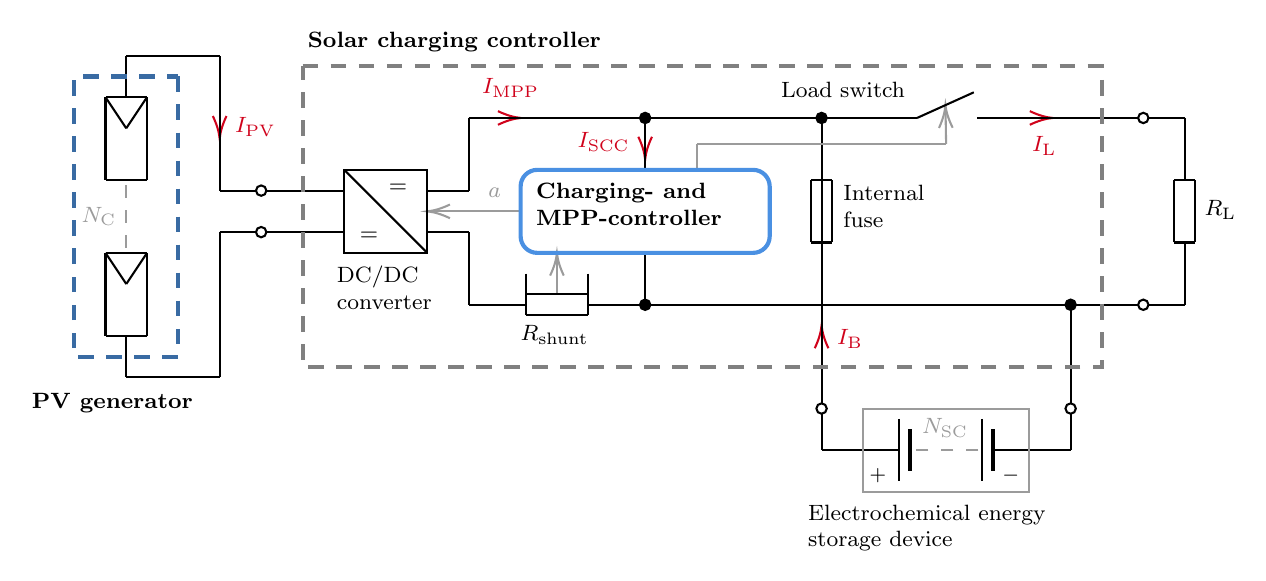
\begin{tikzpicture}[x=0.75pt,y=0.75pt,yscale=-1,xscale=1]
%uncomment if require: \path (0,699); %set diagram left start at 0, and has height of 699

%Straight Lines [id:da9421417995427921] 
\draw [color={rgb, 255:red, 208; green, 2; blue, 27 }  ,draw opacity=1 ]   (340,135) -- (340,148) ;
\draw [shift={(340,150)}, rotate = 270] [color={rgb, 255:red, 208; green, 2; blue, 27 }  ,draw opacity=1 ][line width=0.75]    (10.93,-3.29) .. controls (6.95,-1.4) and (3.31,-0.3) .. (0,0) .. controls (3.31,0.3) and (6.95,1.4) .. (10.93,3.29)   ;
%Straight Lines [id:da11882011111847857] 
\draw [color={rgb, 255:red, 208; green, 2; blue, 27 }  ,draw opacity=1 ]   (265,130) -- (278,130) ;
\draw [shift={(280,130)}, rotate = 180] [color={rgb, 255:red, 208; green, 2; blue, 27 }  ,draw opacity=1 ][line width=0.75]    (10.93,-3.29) .. controls (6.95,-1.4) and (3.31,-0.3) .. (0,0) .. controls (3.31,0.3) and (6.95,1.4) .. (10.93,3.29)   ;
%Straight Lines [id:da5374030929898519] 
\draw [color={rgb, 255:red, 155; green, 155; blue, 155 }  ,draw opacity=1 ]   (297.5,215) -- (297.5,197) ;
\draw [shift={(297.5,195)}, rotate = 450] [color={rgb, 255:red, 155; green, 155; blue, 155 }  ,draw opacity=1 ][line width=0.75]    (10.93,-3.29) .. controls (6.95,-1.4) and (3.31,-0.3) .. (0,0) .. controls (3.31,0.3) and (6.95,1.4) .. (10.93,3.29)   ;
%Straight Lines [id:da1989790363552124] 
\draw [color={rgb, 255:red, 208; green, 2; blue, 27 }  ,draw opacity=1 ]   (521.25,130) -- (534.25,130) ;
\draw [shift={(536.25,130)}, rotate = 180] [color={rgb, 255:red, 208; green, 2; blue, 27 }  ,draw opacity=1 ][line width=0.75]    (10.93,-3.29) .. controls (6.95,-1.4) and (3.31,-0.3) .. (0,0) .. controls (3.31,0.3) and (6.95,1.4) .. (10.93,3.29)   ;
%Straight Lines [id:da21829966681616142] 
\draw [color={rgb, 255:red, 208; green, 2; blue, 27 }  ,draw opacity=1 ]   (425,245) -- (425,232) ;
\draw [shift={(425,230)}, rotate = 450] [color={rgb, 255:red, 208; green, 2; blue, 27 }  ,draw opacity=1 ][line width=0.75]    (10.93,-3.29) .. controls (6.95,-1.4) and (3.31,-0.3) .. (0,0) .. controls (3.31,0.3) and (6.95,1.4) .. (10.93,3.29)   ;
%Straight Lines [id:da03029227215015773] 
\draw [color={rgb, 255:red, 208; green, 2; blue, 27 }  ,draw opacity=1 ]   (135,120) -- (135,138) ;
\draw [shift={(135,140)}, rotate = 270] [color={rgb, 255:red, 208; green, 2; blue, 27 }  ,draw opacity=1 ][line width=0.75]    (10.93,-3.29) .. controls (6.95,-1.4) and (3.31,-0.3) .. (0,0) .. controls (3.31,0.3) and (6.95,1.4) .. (10.93,3.29)   ;
%Straight Lines [id:da02274138666088943] 
\draw    (135,165) -- (135,100) ;
%Straight Lines [id:da9018683092685658] 
\draw [color={rgb, 255:red, 155; green, 155; blue, 155 }  ,draw opacity=1 ]   (365,155) -- (365,142.5) ;
%Straight Lines [id:da3536205977605156] 
\draw [color={rgb, 255:red, 155; green, 155; blue, 155 }  ,draw opacity=1 ]   (484.71,125.83) -- (485,142.5) ;
\draw [shift={(484.67,123.83)}, rotate = 88.99] [color={rgb, 255:red, 155; green, 155; blue, 155 }  ,draw opacity=1 ][line width=0.75]    (10.93,-3.29) .. controls (6.95,-1.4) and (3.31,-0.3) .. (0,0) .. controls (3.31,0.3) and (6.95,1.4) .. (10.93,3.29)   ;
%Straight Lines [id:da3940961623559218] 
\draw [color={rgb, 255:red, 155; green, 155; blue, 155 }  ,draw opacity=1 ] [dash pattern={on 4.5pt off 4.5pt}]  (90,192.5) -- (90,157.5) ;
%Straight Lines [id:da305486791416246] 
\draw    (100,120) -- (80,120) ;
%Straight Lines [id:da18383705888296387] 
\draw    (100,120) -- (90,135) ;
%Straight Lines [id:da3095194315665788] 
\draw    (90,135) -- (80,120) ;
%Straight Lines [id:da698747256222205] 
\draw    (100,120) -- (100,160) ;
%Straight Lines [id:da9106612303236621] 
\draw    (80,120) -- (80,160) ;
%Straight Lines [id:da2775343790641671] 
\draw    (100,160) -- (80,160) ;
%Straight Lines [id:da6238057844394507] 
\draw    (90,235) -- (90,255) ;
%Straight Lines [id:da9446915580972504] 
\draw    (90,100) -- (90,120) ;
%Straight Lines [id:da2886170332859268] 
\draw    (100,195) -- (80,195) ;
%Straight Lines [id:da4973666404379713] 
\draw    (100,195) -- (90,210) ;
%Straight Lines [id:da3822755028621725] 
\draw    (90,210) -- (80,195) ;
%Straight Lines [id:da8935801956358882] 
\draw    (100,195) -- (100,235) ;
%Straight Lines [id:da6312155893729114] 
\draw    (80,195) -- (80,235) ;
%Straight Lines [id:da6010711027940552] 
\draw    (100,235) -- (80,235) ;
%Shape: Rectangle [id:dp6783742410505116] 
\draw  [color={rgb, 255:red, 57; green, 107; blue, 163 }  ,draw opacity=1 ][dash pattern={on 5.63pt off 4.5pt}][line width=1.5]  (115,110) -- (115,245) -- (65,245) -- (65,110) -- cycle ;
%Straight Lines [id:da2862092994413896] 
\draw    (90,100) -- (135,100) ;
%Straight Lines [id:da4924615198515234] 
\draw    (90,255) -- (135,255) ;
%Straight Lines [id:da8029714671125825] 
\draw    (135,185) -- (135,255) ;
%Straight Lines [id:da7764512241735024] 
\draw    (135,165) -- (152.5,165) ;
%Straight Lines [id:da5197356742187318] 
\draw    (135,185) -- (152.5,185) ;
%Shape: Circle [id:dp45159015891408627] 
\draw   (152.5,185) .. controls (152.5,183.62) and (153.62,182.5) .. (155,182.5) .. controls (156.38,182.5) and (157.5,183.62) .. (157.5,185) .. controls (157.5,186.38) and (156.38,187.5) .. (155,187.5) .. controls (153.62,187.5) and (152.5,186.38) .. (152.5,185) -- cycle ;
%Shape: Circle [id:dp8259240874509837] 
\draw   (152.5,165) .. controls (152.5,163.62) and (153.62,162.5) .. (155,162.5) .. controls (156.38,162.5) and (157.5,163.62) .. (157.5,165) .. controls (157.5,166.38) and (156.38,167.5) .. (155,167.5) .. controls (153.62,167.5) and (152.5,166.38) .. (152.5,165) -- cycle ;
%Straight Lines [id:da6710153722448606] 
\draw    (157.5,165) -- (195,165) ;
%Straight Lines [id:da2438484327573136] 
\draw    (157.5,185) -- (195,185) ;
%Straight Lines [id:da014835098389228696] 
\draw    (195,155) -- (235,195) ;
%Straight Lines [id:da591897012695844] 
\draw    (235,185) -- (255,185) ;
%Straight Lines [id:da08002520414789704] 
\draw    (235,165) -- (255,165) ;
%Straight Lines [id:da573801302408715] 
\draw    (255,165) -- (255,130) ;
%Straight Lines [id:da8156706903846436] 
\draw    (255,220) -- (255,185) ;
%Straight Lines [id:da06349281099489246] 
\draw    (255,130) -- (340,130) ;
%Straight Lines [id:da2570308374665804] 
\draw [color={rgb, 255:red, 155; green, 155; blue, 155 }  ,draw opacity=1 ]   (237,175) -- (280,175) ;
\draw [shift={(235,175)}, rotate = 0] [color={rgb, 255:red, 155; green, 155; blue, 155 }  ,draw opacity=1 ][line width=0.75]    (10.93,-3.29) .. controls (6.95,-1.4) and (3.31,-0.3) .. (0,0) .. controls (3.31,0.3) and (6.95,1.4) .. (10.93,3.29)   ;
%Straight Lines [id:da8534254271800685] 
\draw    (340,220) -- (577.5,220) ;
%Straight Lines [id:da6771997897740949] 
\draw    (340,130) -- (340,155) ;
%Straight Lines [id:da4018491949490153] 
\draw    (340,220) -- (340,195) ;
%Shape: Square [id:dp006137277495093407] 
\draw   (195,155) -- (235,155) -- (235,195) -- (195,195) -- cycle ;
%Shape: Circle [id:dp7845577348540074] 
\draw  [fill={rgb, 255:red, 0; green, 0; blue, 0 }  ,fill opacity=1 ] (340,217.5) .. controls (341.38,217.5) and (342.5,218.62) .. (342.5,220) .. controls (342.5,221.38) and (341.38,222.5) .. (340,222.5) .. controls (338.62,222.5) and (337.5,221.38) .. (337.5,220) .. controls (337.5,218.62) and (338.62,217.5) .. (340,217.5) -- cycle ;
%Shape: Circle [id:dp8572849216277822] 
\draw  [fill={rgb, 255:red, 0; green, 0; blue, 0 }  ,fill opacity=1 ] (340,127.5) .. controls (341.38,127.5) and (342.5,128.62) .. (342.5,130) .. controls (342.5,131.38) and (341.38,132.5) .. (340,132.5) .. controls (338.62,132.5) and (337.5,131.38) .. (337.5,130) .. controls (337.5,128.62) and (338.62,127.5) .. (340,127.5) -- cycle ;
%Straight Lines [id:da3780211255481636] 
\draw    (524.5,290) -- (545,290) ;
%Straight Lines [id:da03184575218832286] 
\draw    (425,290) -- (445,290) ;
%Straight Lines [id:da2327687009499042] 
\draw [line width=0.75]    (462.5,275) -- (462.5,305) ;
%Straight Lines [id:da6973962605147832] 
\draw [color={rgb, 255:red, 155; green, 155; blue, 155 }  ,draw opacity=1 ] [dash pattern={on 4.5pt off 4.5pt}]  (500.5,290) -- (465.5,290) ;
%Straight Lines [id:da942581709626162] 
\draw [line width=1.5]    (467.5,280) -- (467.5,300) ;
%Straight Lines [id:da9460540646491606] 
\draw [line width=0.75]    (502.5,275) -- (502.5,305) ;
%Straight Lines [id:da815017798843781] 
\draw [line width=1.5]    (507.5,280) -- (507.5,300) ;
%Straight Lines [id:da591654385387534] 
\draw    (462.5,290) -- (445.5,290) ;
%Straight Lines [id:da9349050114513227] 
\draw    (524.5,290) -- (507.5,290) ;
%Shape: Rectangle [id:dp05962945052172275] 
\draw  [color={rgb, 255:red, 155; green, 155; blue, 155 }  ,draw opacity=1 ] (525,270) -- (525,310) -- (445,310) -- (445,270) -- cycle ;
%Shape: Circle [id:dp15752231467223798] 
\draw  [fill={rgb, 255:red, 0; green, 0; blue, 0 }  ,fill opacity=1 ] (425,127.5) .. controls (426.38,127.5) and (427.5,128.62) .. (427.5,130) .. controls (427.5,131.38) and (426.38,132.5) .. (425,132.5) .. controls (423.62,132.5) and (422.5,131.38) .. (422.5,130) .. controls (422.5,128.62) and (423.62,127.5) .. (425,127.5) -- cycle ;
%Shape: Circle [id:dp5007554014602349] 
\draw   (422.5,270) .. controls (422.5,268.62) and (423.62,267.5) .. (425,267.5) .. controls (426.38,267.5) and (427.5,268.62) .. (427.5,270) .. controls (427.5,271.38) and (426.38,272.5) .. (425,272.5) .. controls (423.62,272.5) and (422.5,271.38) .. (422.5,270) -- cycle ;
%Straight Lines [id:da9208992192503083] 
\draw    (545,272.5) -- (545,290) ;
%Straight Lines [id:da627604798253242] 
\draw    (425,272.5) -- (425,290) ;
%Shape: Circle [id:dp2556214449799865] 
\draw   (542.5,270) .. controls (542.5,268.62) and (543.62,267.5) .. (545,267.5) .. controls (546.38,267.5) and (547.5,268.62) .. (547.5,270) .. controls (547.5,271.38) and (546.38,272.5) .. (545,272.5) .. controls (543.62,272.5) and (542.5,271.38) .. (542.5,270) -- cycle ;
%Straight Lines [id:da6463205767083462] 
\draw    (545,220) -- (545,267.5) ;
%Shape: Circle [id:dp5678761425198426] 
\draw  [fill={rgb, 255:red, 0; green, 0; blue, 0 }  ,fill opacity=1 ] (545,217.5) .. controls (546.38,217.5) and (547.5,218.62) .. (547.5,220) .. controls (547.5,221.38) and (546.38,222.5) .. (545,222.5) .. controls (543.62,222.5) and (542.5,221.38) .. (542.5,220) .. controls (542.5,218.62) and (543.62,217.5) .. (545,217.5) -- cycle ;
%Straight Lines [id:da6220082414399177] 
\draw    (425,130) -- (425,267.5) ;
%Straight Lines [id:da2232912850869122] 
\draw    (430,160) -- (420,160) ;
%Straight Lines [id:da5727217442177441] 
\draw    (430,190) -- (420,190) ;
%Straight Lines [id:da19246645036279175] 
\draw    (430,190) -- (430,160) ;
%Straight Lines [id:da4957674579678937] 
\draw    (420,190) -- (420,160) ;
%Shape: Circle [id:dp7355797988494659] 
\draw   (577.5,220) .. controls (577.5,218.62) and (578.62,217.5) .. (580,217.5) .. controls (581.38,217.5) and (582.5,218.62) .. (582.5,220) .. controls (582.5,221.38) and (581.38,222.5) .. (580,222.5) .. controls (578.62,222.5) and (577.5,221.38) .. (577.5,220) -- cycle ;
%Shape: Circle [id:dp40339619027918716] 
\draw   (577.5,130) .. controls (577.5,128.62) and (578.62,127.5) .. (580,127.5) .. controls (581.38,127.5) and (582.5,128.62) .. (582.5,130) .. controls (582.5,131.38) and (581.38,132.5) .. (580,132.5) .. controls (578.62,132.5) and (577.5,131.38) .. (577.5,130) -- cycle ;
%Straight Lines [id:da634111336257325] 
\draw    (577.5,130) -- (500,130) ;
%Straight Lines [id:da13864177091392604] 
\draw    (498.34,117.65) -- (471,130) ;
%Straight Lines [id:da5827331843556056] 
\draw    (471,130) -- (425,130) ;
%Straight Lines [id:da7062937681829833] 
\draw [color={rgb, 255:red, 155; green, 155; blue, 155 }  ,draw opacity=1 ]   (485,142.5) -- (365,142.5) ;
%Rounded Rect [id:dp5103064937946986] 
\draw  [color={rgb, 255:red, 74; green, 144; blue, 226 }  ,draw opacity=1 ][line width=1.5]  (280,163) .. controls (280,158.58) and (283.58,155) .. (288,155) -- (392,155) .. controls (396.42,155) and (400,158.58) .. (400,163) -- (400,187) .. controls (400,191.42) and (396.42,195) .. (392,195) -- (288,195) .. controls (283.58,195) and (280,191.42) .. (280,187) -- cycle ;
%Shape: Rectangle [id:dp17230778221444543] 
\draw  [color={rgb, 255:red, 128; green, 128; blue, 128 }  ,draw opacity=1 ][dash pattern={on 5.63pt off 4.5pt}][line width=1.5]  (175,105) -- (560,105) -- (560,250) -- (175,250) -- cycle ;
%Straight Lines [id:da888966614057181] 
\draw    (605,160) -- (595,160) ;
%Straight Lines [id:da4674825884766862] 
\draw    (605,190) -- (595,190) ;
%Straight Lines [id:da17325028423110056] 
\draw    (595,190) -- (595,160) ;
%Straight Lines [id:da3187482405619504] 
\draw    (605,190) -- (605,160) ;
%Straight Lines [id:da7972051733354486] 
\draw    (582.5,130) -- (600,130) ;
%Straight Lines [id:da18847306710691814] 
\draw    (600,190) -- (600,220) ;
%Straight Lines [id:da5858572022127997] 
\draw    (600,130) -- (600,160) ;
%Straight Lines [id:da09365392979639964] 
\draw    (582.5,220) -- (600,220) ;
%Straight Lines [id:da17780600814069225] 
\draw    (312.5,225) -- (312.5,215) ;
%Straight Lines [id:da9675828109503861] 
\draw    (282.5,225) -- (282.5,215) ;
%Straight Lines [id:da8123532634949631] 
\draw    (282.5,225) -- (312.5,225) ;
%Straight Lines [id:da8259034059803427] 
\draw    (282.5,215) -- (312.5,215) ;
%Straight Lines [id:da44215658235611977] 
\draw    (255,220) -- (282,220) ;
%Straight Lines [id:da6994883602565676] 
\draw    (313,220) -- (340,220) ;
%Straight Lines [id:da5905851393973105] 
\draw    (340,130) -- (425,130) ;
%Straight Lines [id:da49034677151619577] 
\draw    (282.5,205) -- (282.5,215) ;
%Straight Lines [id:da9931250995037515] 
\draw    (312.5,205) -- (312.5,215) ;

% Text Node
\draw (43,261) node [anchor=north west][inner sep=0.75pt]  [font=\footnotesize] [align=left] {\textbf{PV generator}};
% Text Node
\draw (67,171.4) node [anchor=north west][inner sep=0.75pt]  [font=\footnotesize,color={rgb, 255:red, 155; green, 155; blue, 155 }  ,opacity=1 ]  {$N_{\mathrm{C}}$};
% Text Node
\draw (215,160.4) node [anchor=north west][inner sep=0.75pt]  [font=\footnotesize]  {$=$};
% Text Node
\draw (201,183.4) node [anchor=north west][inner sep=0.75pt]  [font=\footnotesize]  {$=$};
% Text Node
\draw (286,160) node [anchor=north west][inner sep=0.75pt]  [font=\footnotesize] [align=left] {\textbf{Charging- and }\\\textbf{MPP-controller}};
% Text Node
\draw (263,162.4) node [anchor=north west][inner sep=0.75pt]  [font=\footnotesize,color={rgb, 255:red, 155; green, 155; blue, 155 }  ,opacity=1 ]  {$a$};
% Text Node
\draw (510.5,297.4) node [anchor=north west][inner sep=0.75pt]  [font=\scriptsize]  {$-$};
% Text Node
\draw (446.5,297.4) node [anchor=north west][inner sep=0.75pt]  [font=\scriptsize]  {$+$};
% Text Node
\draw (472,273.4) node [anchor=north west][inner sep=0.75pt]  [font=\footnotesize,color={rgb, 255:red, 155; green, 155; blue, 155 }  ,opacity=1 ]  {$N_{\mathrm{SC}}$};
% Text Node
\draw (176,87) node [anchor=north west][inner sep=0.75pt]  [font=\footnotesize] [align=left] {\textbf{Solar charging controller}};
% Text Node
\draw (404,111) node [anchor=north west][inner sep=0.75pt]  [font=\footnotesize] [align=left] {Load switch};
% Text Node
\draw (434,161) node [anchor=north west][inner sep=0.75pt]  [font=\footnotesize] [align=left] {Internal\\fuse};
% Text Node
\draw (141,128.4) node [anchor=north west][inner sep=0.75pt]  [font=\footnotesize,color={rgb, 255:red, 208; green, 2; blue, 27 }  ,opacity=1 ]  {$I_{\mathrm{PV}}$};
% Text Node
\draw (431,230.4) node [anchor=north west][inner sep=0.75pt]  [font=\footnotesize,color={rgb, 255:red, 208; green, 2; blue, 27 }  ,opacity=1 ]  {$I_{\mathrm{B}}$};
% Text Node
\draw (417,315) node [anchor=north west][inner sep=0.75pt]  [font=\footnotesize] [align=left] {Electrochemical energy\\storage device};
% Text Node
\draw (525,137.4) node [anchor=north west][inner sep=0.75pt]  [font=\footnotesize,color={rgb, 255:red, 208; green, 2; blue, 27 }  ,opacity=1 ]  {$I_{\mathrm{L}}$};
% Text Node
\draw (608,168.4) node [anchor=north west][inner sep=0.75pt]  [font=\footnotesize]  {$R_{\mathrm{L}}$};
% Text Node
\draw (278.5,228.4) node [anchor=north west][inner sep=0.75pt]  [font=\footnotesize]  {$R_{\mathrm{shunt}}$};
% Text Node
\draw (306,135.4) node [anchor=north west][inner sep=0.75pt]  [font=\footnotesize,color={rgb, 255:red, 208; green, 2; blue, 27 }  ,opacity=1 ]  {$I_{\mathrm{SCC}}$};
% Text Node
\draw (260,109.4) node [anchor=north west][inner sep=0.75pt]  [font=\footnotesize,color={rgb, 255:red, 208; green, 2; blue, 27 }  ,opacity=1 ]  {${I_{\mathrm{MPP}}}$};
% Text Node
\draw (190,200) node [anchor=north west][inner sep=0.75pt]  [font=\footnotesize] [align=left] {DC/DC\\converter};


\end{tikzpicture}

	\caption{The basic structure of a maximum power point tracking solar charging controller. (Recreated from: \cite{Mertens:2015})}
	\label{fig:tikz_SCC}
\end{figure}



